% The Bridge Experiment — report VERSION 2, DRAFT edition.
% Source of truth: docs/research/BRIDGE-REPORT.md (v2 draft, converted 2026-08-01).
% This is the PRE-adversarial-review draft: every page is watermarked DRAFT and
% two data slots remain open ([[SLOT:JUDGE]] in §5, [[SLOT:UNION]] in §6.3),
% typeset as framed "Pending" boxes. Do not cite.
% The archived v1 edition is report.tex / report.pdf — do not modify those.
% Figures included: fig5_tooluse.pdf (telemetry, unchanged by the corrections)
% and fig3_retrieval.pdf (point estimates unchanged; caption notes the redone
% declaration-level CIs). fig1/fig2/fig4 are pre-repair and deliberately omitted.
% Build: latexmk -pdf draft-v2.tex
\documentclass[10pt]{article}

\usepackage[margin=1in,headheight=14.5pt]{geometry}
\usepackage[T1]{fontenc}
\usepackage[utf8]{inputenc}
\usepackage{lmodern}
\usepackage{microtype}
\usepackage{booktabs}
\usepackage{longtable}
\usepackage{graphicx}
\usepackage{amsmath,amssymb}
\usepackage{array}
\usepackage{enumitem}
\usepackage{xcolor}
\usepackage{fancyhdr}
\usepackage{draftwatermark}
\usepackage{tcolorbox}
\tcbuselibrary{breakable}
\usepackage[hidelinks]{hyperref}
\urlstyle{tt}

% --- DRAFT dressing: diagonal watermark + gray running header on every page ---
\SetWatermarkText{DRAFT}
\SetWatermarkScale{1.1}
\SetWatermarkLightness{0.92}
\pagestyle{fancy}
\fancyhf{}
\fancyhead[C]{\color{black!45}\small\textsc{draft v2 --- pre-review, two data slots open}}
\fancyfoot[C]{\thepage}
\renewcommand{\headrulewidth}{0pt}
\fancypagestyle{plain}{%
  \fancyhf{}%
  \fancyhead[C]{\color{black!45}\small\textsc{draft v2 --- pre-review, two data slots open}}%
  \fancyfoot[C]{\thepage}%
  \renewcommand{\headrulewidth}{0pt}}

% --- Pending-slot boxes for the two open [[SLOT]] placeholders ---
\newtcolorbox{pendingbox}[1]{breakable, colback=black!4, colframe=black!55,
  boxrule=0.9pt, arc=1.5pt, title={#1}, fonttitle=\bfseries,
  colbacktitle=black!12, coltitle=black,
  left=7pt, right=7pt, top=6pt, bottom=6pt}

\setlist{itemsep=2pt,topsep=3pt,parsep=0pt}
\setlength{\emergencystretch}{2.5em}
\tolerance=2000
\newcommand{\code}[1]{\texttt{#1}}
\newcommand{\best}[1]{\textbf{#1}}

\title{\textbf{The Bridge Experiment: Does an Informal$\leftrightarrow$Formal
Join Move End-Task Lean Performance?}}
\author{Jack McCarthy\\
\normalsize WikiLean \,$\cdot$\, \url{https://wikilean.jackmccarthy.org}\\
\normalsize with experiments executed by Claude Code agents under direction}
\date{Report, version 2 (\textbf{DRAFT}) --- July 31, 2026 --- post-review
corrected edition}

\begin{document}
\maketitle
\thispagestyle{plain}

\begin{center}
\fcolorbox{black!55}{black!6}{\begin{minipage}{0.9\textwidth}
\small\centering
\textbf{DRAFT --- pre-adversarial-review edition.} Two data slots are open:
the blind-judge equivalence tables (\S5) and the bare-union ablation
(\S6.3). Not for citation.
\end{minipage}}
\end{center}

\begin{center}
\begin{minipage}{0.92\textwidth}
\small
Preregistration: \code{docs/research/BRIDGE-EXPERIMENT.md},\\
commit \code{0d36f2664ab2ebb2c7b80b350d3c9bd820414335} (2026-07-16).
Version 1 of
this report (2026-07-25) received an external methodological review on
2026-07-27 (\code{docs/research/review/REVIEW-1.md}); we verified its
factual claims independently
(\code{docs/research/review/verification-of-review-1.json}: 29 confirmed,
1 partial, 1 refuted) and this edition incorporates the corrections.
Version 1 remains in git history. All data, code, and run transcripts are
preserved in the private repository \code{Deicyde/wikilean-bridge-experiment}
(file map in \S11). Every number below is recomputable from a file in that
repository; the file is named where each table appears.
\end{minipage}
\end{center}

\paragraph{How to read this report.} Every result carries one of three
registers, marked at the section or table where it appears:

\begin{itemize}
\item \textbf{[PREREGISTERED-MODIFIED]} --- a preregistered analysis executed
  with a named modification (the modification is stated where the tag
  appears).
\item \textbf{[EXPLORATORY]} --- not preregistered: all of Bridge v2
  (retrieval, SorryDB, tool-use analysis) and the uncalibrated-judge grading.
\item \textbf{[CORRECTIVE]} --- a reanalysis finding of this edition (error
  repair, exposure audit, cluster-aware statistics).
\end{itemize}

\textbf{Zero results in this report are cleanly confirmatory} under the
preregistered success criterion: that criterion was D$>$E on
\emph{faithful@budget} (semantic equivalence to gold $\wedge$ typecheck) and
D$\leq$E on tokens-to-solve, and neither half was ever graded as specified
(\S3). The uncalibrated-judge section (\S5) is the exploratory substitute
for the missing equivalence leg.

\section{Abstract}\label{sec:abstract}

We test whether a curated dictionary between mathematical concepts and
Mathlib declarations (the WikiLean ``Brain'') improves language-model
performance on formalization tasks, against controls holding the underlying
corpora without the join. Results fall in three registers: one
preregistered-but-modified comparison, a set of exploratory follow-ups, and
the corrective reanalyses prompted by an external review; nothing here is
cleanly confirmatory, because the preregistered semantic-equivalence
endpoint was never graded as specified. Our primary metric is therefore the
\textbf{grounded typecheck rate} --- produced declaration, zero hallucinated
citations, passing typecheck --- which does not measure semantic
correctness. On 100 post-Brain-index tasks (held out from the Brain's
indexes, but not --- we later verified --- from the formal-search arms'
sources), the bundled Wikibrain arm reaches 40.6\% against 23.2\% for the
unjoined-tools control on the 69 completed pairs (McNemar 18/6, exact
$p=0.023$, risk difference $+17.4$pp $[+4.1, +30.7]$); after repairing the
control's 31 infrastructure-failed runs, the full-100 contrast is 42.0\%
vs.\ 30.0\% ($p=0.073$, RD $+12.0$pp $[+0.2, +23.8]$). Join-specific
attribution awaits a factorial ablation; the clean independent finding is
the existence verifier, which cuts hallucinated citations to 6.8\% against
17.7--21.2\% in every other arm. Exploratory results: a post-hoc,
benchmark-informed union-plus-manual agent obtained the highest rows we
observed on MathlibQR-810 and MathlibMPR (declaration-clustered CIs exclude
the single-arm baselines); on SorryDB, kernel-verified proving with and
without the Brain is statistically indistinguishable (10 vs.\ 9 of 171,
$p=1.0$).

\section{The system under test: the WikiLean Brain}\label{sec:system}

The artifact everything below measures is the WikiLean ``Brain'': a curated
knowledge graph over mathematics that joins Wikipedia/Wikidata concepts,
Mathlib4 declarations, and the external mathematical databases (nLab,
LMFDB, the Stacks project, ProofWiki, and others) into one map. Its atom is
a \emph{cell}: when a Lean declaration, a Wikidata concept, an encyclopedia
article, and a database page all denote the same mathematical object, they
are \emph{organs} of one cell rather than separate nodes --- Mathlib's
\code{Module}, Wikidata's ``module'' \emph{and} its ``vector space'' are a
single atom, because Mathlib has no \code{VectorSpace}; \code{Module}
generalizes it. Mathlib's folder hierarchy supplies the containment
altitude, and everything known about a cell (Lean source, descriptions,
licensed database snippets) is embedded on the cell itself. About 12{,}000
of Mathlib's declarations are concept-joined this way; the Brain is a map
of Mathlib, not the territory.

Agents reach it through an MCP server (\code{POST /mcp} on the live site)
exposing eight tools. \code{brain\_bridge} is the informal$\to$formal entry
point: free text in, existence-verified declarations out, each with its
signature, import line, and bond quality. \code{brain\_search} resolves
labels and aliases to atoms; \code{brain\_cell} returns the full atom card;
\code{brain\_transfer} makes the one-atom informal$\leftrightarrow$formal
jump; \code{brain\_neighborhood} walks the synapse graph;
\code{brain\_snippets} and \code{brain\_filter} serve stored content and
facet queries. The eighth, \code{decl\_exists}, is different in kind: a
batch existence check against the full declaration index --- all of
Mathlib, not just the joined subset --- built to be called on every name an
agent is about to cite. It matters below that \code{decl\_exists} queries
(effectively) the same doc-gen4 oracle our scorer uses to grade
hallucinated citations: the bundle contains a tool aimed at a component of
its own score, which is one reason this report no longer attributes effects
to ``the join'' (\S3, \S9).

Why build such a thing? The working hypothesis behind WikiLean is that
informal mathematics (what things are called and mean) and formal
mathematics (what typechecks) are two corpora whose \emph{join} is the
scarce artifact: a language model already holds both corpora loosely, and
the informal$\leftrightarrow$formal boundary is precisely where its
hallucinations live. If that is right, then curating the join --- names
verified, concepts merged, bonds carrying provenance --- should move
performance on end tasks, not just on lookup. Whether it actually does is
the question this report tries, and in this edition only partly manages, to
answer.

\section{Preregistered design and what actually ran}\label{sec:design}

\paragraph{Hypothesis (operationalized).} Since ``necessary'' is unprovable,
the preregistration commits to three predictions. P1: an agent with the
\emph{joined} dictionary beats an agent given informal and formal search
\emph{separately}. P2: the bridge solves at lower cost. P3: the bridge
lifts grounding (fewer hallucinated declaration citations), not just
compile rate. The preregistered success criterion: D$>$E on faithful@budget
($p<.05$) AND D$\leq$E on tokens-to-solve.

\paragraph{The five arms.} All five arms share the same model, prompt, and
budgets within each phase; the only thing that differs between them is the
tool manifest (\code{bench/run\_bridge.py}, manifests in
\code{bench/arms/}); see Table~\ref{tab:arms}.

\begin{table}[htbp]
\centering
\small
\begin{tabular}{@{}lp{0.40\textwidth}p{0.30\textwidth}@{}}
\toprule
Arm & Tools & Intended to isolate \\
\midrule
A \code{no\_tools} & none (\code{--tools ""}) & floor / memorization \\
B \code{informal} & Wikipedia + nLab search/fetch, no Lean mapping & informal reasoning alone \\
C \code{formal} & loogle + ripgrep + source read over a Mathlib checkout & the LeanSearch-class status quo \\
D \code{wikibrain} & the Brain MCP (\code{brain\_bridge}\slash\code{search}\slash\code{cell}\slash\code{transfer}\slash\code{neighborhood}\slash\code{snippets}\slash\code{filter} + batch \code{decl\_exists}) & the join \textbf{+ the existence verifier} (not separable in this design) \\
E \code{B+C unjoined} & B's tools AND C's tools, no join & the unjoined control \\
\bottomrule
\end{tabular}
\caption{The five preregistered arms. Identical model, prompt, and budgets
within each phase; only the tool manifest differs.}
\label{tab:arms}
\end{table}

Two design facts the review surfaced, now stated up front. First, D is the
only arm holding \code{decl\_exists}, and hallucination-free citation is a
conjunct of the primary metric, so D vs.\ E measures the \emph{bundled
Wikibrain package}, not the join per se (on the 100 fresh tasks D made 715
\code{decl\_exists} call attempts, 682 successful). Second, arm E failed
its manipulation check as an ``actively consulting both corpora'' control:
across its 100 fresh runs it touched the informal tools 4 times, against
arm B's 345 --- E behaved as a formal-search agent with a larger manifest
(\code{verification-of-review-1.json}, arm-design section).

{\sloppy
\paragraph{Models per phase.} Tier 1 uses \code{claude-haiku-4-5} (model id
\code{claude-haiku-4-5-20251001}) in all five arms. Bridge v2 (retrieval
and proving) uses \code{claude-sonnet-5} in all agent arms, per a
pre-execution decision (\code{docs/research/BRIDGE-V2-BENCHMARKS.md}). One
model per phase, one seed per (task, arm): a bridge that only helps some
capability band would not be distinguished, and no run-to-run variance is
measured anywhere.\par}

\paragraph{Grading.} The primary metric of this report is the
\textbf{grounded typecheck rate}: the fraction of tasks where the run
produced a declaration, cited zero names absent from a union oracle
(doc-gen4 declaration data $\cup$ verified renames; extractor documented in
\code{bench/score\_bridge.py}), and the declaration typechecked on the
pinned toolchain.\footnote{Version 1 called this metric ``success
(folded)''. The rename follows the external review: a metric with no
semantic-equivalence leg should not be called success.} It is a
syntactic-validity + grounding measure. It does \textbf{not} establish that
the produced statement formalizes the informal prompt: a declaration can
pass all three legs while being weaker, stronger, vacuous, or about the
wrong object. The preregistered faithful@budget (BEq+ equivalence to gold)
was never graded --- the equivalence leg in \code{score\_bridge.py} is a
stub returning \code{None} --- and \S5 holds the exploratory substitute.

\paragraph{Task sets.} Tier 1a is ProofNet\#: 371 problems (341 eval + 30
prompt-freezing dev), pinned to \code{PAug/ProofNetSharp}
@\code{a8da405fbd1e348a87445c2e562c747b7e26dc8f} (MIT; arXiv:2406.07222),
graded on Lean v4.32.0-rc1 / Mathlib \code{a33a5ccd}. Tier 1b is the
\textbf{post-Brain-index fresh set}\footnote{Version 1 called this set
``contamination-proof'' and ``newer than every arm's index''. Both
phrasings are retracted (\S9, concern 4).}: 100 tasks built from theorems
merged into Mathlib master between 2026-07-03 and 07-16, verified absent
from the Brain's declaration universe and node set --- the indexes arm D
serves (\code{bench/data/fresh\_tasks.stats.json}) --- and graded on Lean
v4.33.0-rc1 / Mathlib \code{9944fe29}. The set was \textbf{not} verified
absent from the formal-search arms' sources: arms C/E read a mutable local
checkout (which stood at \code{61a5e4f338}, content through
${\sim}$2026-07-10, during the runs) and queried the live unsnapshotted
Loogle service. \S4.4 measures the resulting exposure directly. A
determinacy pre-screen was preregistered (exclude tasks two independent
formalizers cannot pin down); what ran instead was a post-hoc double
annotation (agreement 79\%, $\kappa\approx0.20$) defining a 74-task
both-determinate subset --- no tasks were excluded.

\paragraph{Budgets and execution.} Every arm ran under a 10-minute wall
clock (enforced) and a 30-turn budget that was \textbf{advisory only} ---
the prompt stated it, but the CLI passed no turn cap. Fresh-set overruns:
C 50 runs, D 38, E 32 exceeded 30 turns, with maxima 80, 88, and 72. The
fresh arms also ran in strictly sequential blocks on 2026-07-19
(A 01:50--02:08Z, B 02:09--03:56Z, C 03:58--04:27Z, D 04:29--04:54Z,
E 04:56--05:17Z) --- no interleaving, so arm is confounded with time of
execution. Agents had no in-loop typechecker and were instructed to verify
cited names through their tools.

\paragraph{The arm-E 429 incident and repair [CORRECTIVE].} Arm E's fresh
block died at its tail: rows fresh\_069--099 (31 contiguous tasks) all
errored with session-limit 429s --- an infrastructure failure at the end of
the sequential E block, not agent behavior. Version 1 scored these as
``produced no declaration'' and read them as evidence that unjoined tool
volume is harmful; that reading is retired. On 2026-07-27 the 31 rows were
rerun (\code{bench/analysis/rerun\_E\_fresh.py}) with E's exact July-19
code path, on a read-only \code{git archive} extraction of
\code{61a5e4f338} --- the same tree content the original C/E runs saw. The
repair surfaced a second condition-fidelity hazard worth recording: under
concurrent cold starts, the CLI's stdio MCP servers can silently fail to
connect, yielding runs that \emph{look} like completions but had zero
tools. The repair driver detects this from the stream-json init event and
forces such rows to error-and-retry rather than recording fake tool-less
completions (commit \code{19a90209}). Originals are archived in
\code{bench/data/runs\_E\_fresh\_429\_archive/}; 14 of the 31 repaired rows
became grounded-typecheck passes
(\code{bench/analysis/bridge\_summary\_v2.json}, \code{v2\_provenance}).

\paragraph{The complete execution table.} Every preregistered component,
its status, and the inferential consequence. (Sources: the
preregistration; the claim-by-claim inventory in
\code{verification-of-review-1.json}, prereg section.)

{\footnotesize
\begin{longtable}{@{}p{0.245\textwidth}p{0.105\textwidth}p{0.315\textwidth}p{0.245\textwidth}@{}}
\toprule
Preregistered component & Status & What actually happened & Inferential consequence \\
\midrule
\endfirsthead
\toprule
Preregistered component & Status & What actually happened & Inferential consequence \\
\midrule
\endhead
\bottomrule
\endfoot
\bottomrule
\endlastfoot
Five arms A--E, identical model/prompt/budget, tools-only difference & executed & 471 rows/arm (\code{bench/data/runs/}) & design intact \\
Per-tool call logging & executed & \code{tool\_calls\_by\_name} every row; full traces eval C/D/E + fresh (deviation 7) & enables \S4.5 attribution \\
Tier 1a ProofNet\# (371) & executed & 371/arm, scored & contaminated by construction (arm A 59.8\% on eval-341); paired deltas only \\
Tier 1b fresh set (${\sim}$100) & executed & 100 tasks & holdout guarantee narrower than claimed (Brain indexes only) --- renamed post-Brain-index \\
Hallucinated-decl rate & executed & all tables & the cleanest surviving mechanism signal \\
McNemar D-vs-E / D-vs-C + discordant tables & executed & \S4 & run on grounded typecheck, not the preregistered endpoint \\
10-min wall clock & executed & 600\,s timeouts & --- \\
Pre-campaign API requirements 1--8 & executed & implemented before campaign & --- \\
30-turn budget & \textbf{modified} & advisory only; overruns C 50/D 38/E 32, max 88 & budget is uncontrolled; \S4.3 sensitivity analysis \\
Determinacy pre-screen (exclude) & \textbf{modified} & post-hoc dual annotation (79\%, $\kappa\approx0.20$); 74-task subset, none excluded & subset analysis, not screened population \\
Arm-D production server & \textbf{modified} & production Worker code served locally over shipped shards (deviation 2) & none material \\
Single-shot elaboration grading & \textbf{modified} & persistent REPL, same pins (deviation 3) & none material \\
$\leq$4 typecheck calls in-loop & \textbf{modified} & no in-loop typechecking at all (deviation 4) & halluc rate is a pure grounding measure \\
Skill/ToolSearch leak & \textbf{modified} & sealed before eval; 120 dev runs quarantined (deviation 6) & dev split discarded, eval clean \\
Per-arm cost distributions & \textbf{modified} & means only (USD + wall-clock) & descriptive \\
faithful@budget (BEq+ equivalence) & \textbf{not executed} & grader is a stub; zero judge files in campaign & primary endpoint missing; no confirmatory claim possible \\
LLM judge + 50-item human calibration & \textbf{not executed} (campaign) & harness existed unused; an \emph{uncalibrated} blind judge pass was launched post-review (\S5) & \S5 is exploratory only \\
tokens-to-solve (half the success criterion) & \textbf{not executed} & never computed (tokens recorded per row) & P2 untested as specified \\
3 reseeds + pass@k curves & \textbf{not executed} & one run per (task, arm) everywhere & no variance estimate; single-seed caveat on every number \\
Second model class on primary set & \textbf{not executed} & Tier-1 all-Haiku; v2 all-Sonnet on different benchmarks & capability-band generality unknown \\
Preregistered success criterion & \textbf{not executed} & neither half graded as specified & zero confirmatory results \\
Tier 2 as specified (FATE-H + MPR-Prop proving, reflection loop, arms A/C/D/E) & \textbf{not executed} & replaced by exploratory v2: QR/MPR retrieval + one-shot SorryDB, arms N/F/W/WF & \S\S6--7 are exploratory, not the preregistered Tier 2 \\
PutnamBench & \textbf{not executed} & --- & --- \\
Tier 3a offline Erd\H{o}s set & \textbf{not executed} & --- & --- \\
Tier 3b live Erd\H{o}s queue & \textbf{not executed} & --- & --- \\
\end{longtable}
}

\section{Tier 1: statement autoformalization (claude-haiku-4-5)}\label{sec:tier1}

\textbf{[PREREGISTERED-MODIFIED]} --- the preregistered paired design,
graded on grounded typecheck rate instead of faithful@budget, one model,
one seed, advisory turn budget. Corrected tables below are from
\code{bench/analysis/tier1\_reanalysis.\{json,md\}} and
\code{bench/analysis/part1\_fresh100\_v2.\{json$\to$bridge\_summary\_v2.json,md\}};
all rates carry Wilson 95\% CIs.

\subsection{Tier 1a --- ProofNet\# eval split (n=341/arm)}\label{sec:tier1a}

\begin{center}
\small
\begin{tabular}{@{}lll@{}}
\toprule
arm & grounded typecheck & Wilson 95\% CI \\
\midrule
A none & 204/341 = 59.8\% & [54.5, 64.9] \\
B wiki & 198/341 = 58.1\% & [52.8, 63.2] \\
C formal & 218/341 = 63.9\% & [58.7, 68.9] \\
D wikibrain & 219/341 = 64.2\% & [59.0, 69.1] \\
E B+C unjoined & 208/341 = 61.0\% & [55.7, 66.0] \\
\bottomrule
\end{tabular}
\end{center}

The arms sit within a few points of each other; the v1 D-vs-E McNemar
(63 vs.\ 51 discordant over the 371 folded pairs, exact $p=0.30$) is an
underpowered null. Arm A at ${\sim}$60\% with zero tools is substantial
ProofNet memorization and was the motivation for Tier 1b. The
typecheck-only row still \emph{anti-correlates} with grounding (E led
typecheck at 83.3\% while trailing on hallucinations in the v1 tables) ---
reproducing TheoremGraph's typecheck-is-not-a-signal finding at $15\times$
their $n$. Tier-1a is contaminated by construction; we report it for the
paired deltas and as the memorization control, never alone.

\subsection{Tier 1b --- the post-Brain-index fresh set (n=100/arm)}\label{sec:tier1b}

Three analyses, in order of increasing completeness. First, the campaign
as it actually ran, with E's 31 infrastructure-dead rows counted as
failures (intention-to-treat over the snapshot;
\code{tier1\_reanalysis.md} \S2):

\begin{center}
\small
\begin{tabular}{@{}lllc@{}}
\toprule
arm & grounded typecheck & Wilson 95\% CI & infra errors \\
\midrule
A & 20/100 = 20.0\% & [13.3, 28.9] & 0 \\
B & 22/100 = 22.0\% & [15.0, 31.1] & 0 \\
C & 25/100 = 25.0\% & [17.5, 34.3] & 0 \\
D & 42/100 = 42.0\% & [32.8, 51.8] & 0 \\
E & 16/100 = 16.0\% & [10.1, 24.4] & \textbf{31} \\
\bottomrule
\end{tabular}
\end{center}

E's row conflates agent behavior with a rate-limit outage; the D-vs-E
McNemar on this table is the error-inflated figure v1 headlined, and it now
appears only in \S9. The two contrasts \emph{unaffected} by the outage
(their arms had zero errors): \textbf{D vs.\ C 28/11 discordant, exact
$p = 0.0095$; D vs.\ A 29/7, $p = 0.0003$} (100 pairs each).

Second, the completed-pairs analysis --- the 69 tasks arm E actually ran
--- which is this report's headline Tier-1 contrast
(\code{tier1\_reanalysis.md} \S3, \S6):

\begin{center}
\small
\begin{tabular}{@{}lll@{}}
\toprule
arm & grounded typecheck (n=69) & Wilson 95\% CI \\
\midrule
A & 10/69 = 14.5\% & [8.1, 24.7] \\
B & 12/69 = 17.4\% & [10.2, 28.0] \\
C & 12/69 = 17.4\% & [10.2, 28.0] \\
D & \best{28/69 = 40.6\%} & [29.8, 52.4] \\
E & 16/69 = 23.2\% & [14.8, 34.4] \\
\bottomrule
\end{tabular}
\end{center}

\textbf{D vs.\ E: McNemar 18/6 discordant, exact $p = 0.023$; risk
difference $+17.4$pp, 95\% CI $[+4.1, +30.7]$} (paired Wald). Also D vs.\ C
21/5, $p=0.0025$; D vs.\ A 22/4, $p=0.0005$ on these pairs.

Third, the post-repair full 100 --- all 500 fresh rows completed, the 31
repaired E rows scored with the identical pipeline
(\code{bench/analysis/part1\_fresh100\_v2.md}, from
\code{bridge\_summary\_v2.json}):

\begin{center}
\small
\begin{tabular}{@{}lll@{}}
\toprule
arm & grounded typecheck (n=100) & Wilson 95\% CI \\
\midrule
A & 20/100 = 20.0\% & [13.3, 28.9] \\
B & 22/100 = 22.0\% & [15.0, 31.1] \\
C & 25/100 = 25.0\% & [17.5, 34.3] \\
D & \best{42/100 = 42.0\%} & [32.8, 51.8] \\
E & 30/100 = 30.0\% & [21.9, 39.6] \\
\bottomrule
\end{tabular}
\end{center}

\textbf{D vs.\ E post-repair: McNemar 25/13, exact $p = 0.073$; RD
$+12.0$pp, 95\% CI $[+0.2, +23.8]$.} D vs.\ C ($p=0.0095$) and D vs.\ A
($p=0.0003$) are unchanged --- only E's cells moved. Stated plainly: with
the infrastructure failures repaired, the bundled-Wikibrain-vs-unjoined
contrast on the full set is a directionally consistent but marginal effect
(the RD interval barely excludes zero; the McNemar $p$ does not reach
0.05); the completed-pairs contrast is significant. And E, repaired, is an
unremarkable mid-pack arm (30\%, statistically indistinguishable from C,
$p=0.42$): version 1's ``unjoined tool volume can be actively harmful'' was
an infrastructure artifact and is retired.

Arm A's collapse from 59.8\% (1a) to 20\% here remains the cleanest
memorization quantification in the study.

\subsection{Turn-budget sensitivity [CORRECTIVE]}\label{sec:budget}

The 30-turn budget was advisory (\S3), so we recompute restricted to pairs
where \textbf{both} arms stayed within 30 turns (snapshot outcomes;
\code{tier1\_reanalysis.md} \S5). D vs.\ E: $n=45$ pairs, D 46.7\%
[32.9, 60.9] vs.\ E 24.4\% [14.2, 38.7], 16 discordant, $p = 0.021$ --- but
this error-inclusive version counts E's 429 rows (turns=1) as within-budget
failures. The honest completed-only version is underpowered: $n=27$ pairs,
D 44.4\% [27.6, 62.7] vs.\ E 40.7\% [24.5, 59.3], 7 discordant, $p = 1.0$.
D vs.\ C within budget: $n=35$, D 54.3\% [38.2, 69.5] vs.\ C 25.7\%
[14.2, 42.1], 12 discordant, $p = 0.0063$. The budget-restricted evidence
is consistent in direction and, for D-vs-E, inconclusive once both
restrictions are applied at once.

\subsection{Exposure strata: what the formal-search leak actually touched
[CORRECTIVE]}\label{sec:exposure}

The review found the fresh golds were not held out from arms C/E's
sources. We measured it (\code{bench/analysis/fresh\_exposure.\{json,md\}};
read-only \code{git archive} of the pinned tree \code{61a5e4f338}, content
date 2026-07-10). Of the 100 tasks: the gold's full dotted name appears
verbatim somewhere in the tree for \textbf{37}; the basename appears as a
declaration header anywhere for \textbf{64}; the basename appears as a
declaration header \textbf{in the task's own module file} for \textbf{51}
--- the exposure basis used below; and the gold's commit is an ancestor of
the pin for 49.\footnote{Exposure is measured on tree bytes, not merge
metadata: two tasks (\code{fresh\_037}, \code{fresh\_054}) are exposed
despite post-pin added-commits --- \code{fresh\_054}'s full dotted name
already sits in its module file at the pin --- which is why 51 exposed
$\neq$ 49 merged-before-pin.}

Split outcomes (snapshot basis: E's 429 rows count as failures, so E's
unexposed cell is heavily infrastructure-depressed; the attempted-only rows
exclude them):

Exposed stratum ($n=51$):

\begin{center}
\small
\begin{tabular}{@{}lll@{}}
\toprule
arm & grounded typecheck & Wilson 95\% CI \\
\midrule
A & 9/51 = 17.6\% & [9.6, 30.2] \\
B & 8/51 = 15.7\% & [8.2, 28.0] \\
C & 11/51 = 21.6\% & [12.5, 34.6] \\
D & \best{24/51 = 47.1\%} & [34.1, 60.5] \\
E & 12/51 = 23.5\% & [14.0, 36.8] \\
E attempted-only & 12/44 = 27.3\% & [16.4, 41.9] \\
\bottomrule
\end{tabular}
\end{center}

Unexposed stratum ($n=49$):

\begin{center}
\small
\begin{tabular}{@{}lll@{}}
\toprule
arm & grounded typecheck & Wilson 95\% CI \\
\midrule
A & 11/49 = 22.4\% & [13.0, 35.9] \\
B & 14/49 = 28.6\% & [17.8, 42.4] \\
C & 14/49 = 28.6\% & [17.8, 42.4] \\
D & \best{18/49 = 36.7\%} & [24.7, 50.7] \\
E & 4/49 = 8.2\% & [3.2, 19.2] \\
E attempted-only & 4/25 = 16.0\% & [6.4, 34.6] \\
\bottomrule
\end{tabular}
\end{center}

McNemar by stratum: D vs.\ E exposed 15/3, $p=0.0075$; \textbf{D vs.\ E
unexposed 17/3, $p=0.0026$}. D vs.\ C exposed 18/5, $p=0.0106$; D vs.\ C
unexposed 10/6, $p=0.45$.

The reading has two honest halves. Against E, the leak cannot explain D's
edge: the leak's direction favors C/E (direct source access to the golds;
D's Brain indexes genuinely predate every gold), and D's advantage over E
is \emph{strongest exactly where there was nothing to leak} --- 36.7\%
vs.\ 8.2\% on unexposed tasks (with the caveat that E's unexposed
denominator is the most outage-damaged stratum; even attempted-only, 36.7\%
vs.\ 16.0\%). Against C the picture is weaker: D's edge concentrates in the
exposed stratum and is a null ($p=0.45$) on unexposed tasks --- consistent
with D's advantage over pure formal search depending partly on targets a
formal-search agent could in principle have found in-tree but didn't.

\subsection{Hallucinated citations and trace attribution}\label{sec:halluc}

Hallucination rates on the fresh set, all 100 rows per arm (post-repair;
recomputed for this edition from
\code{bench/data/runs/\{A..E\}/fresh\_*.json} with
\code{score\_bridge.py}'s union oracle):

\begin{center}
\small
\begin{tabular}{@{}lllc@{}}
\toprule
arm & halluc-decl rate (cited names) & runs w/ $\geq$1 hallucination & Wilson 95\% CI (runs, $n=100$) \\
\midrule
A & 94/443 = 21.2\% & 54 & [44.3, 63.4] \\
B & 76/429 = 17.7\% & 48 & [38.5, 57.7] \\
C & 108/517 = 20.9\% & 49 & [39.4, 58.7] \\
D & \best{32/472 = 6.8\%} & \best{23} & [15.8, 32.2] \\
E & 107/505 = 21.2\% & 49 & [39.4, 58.7] \\
\bottomrule
\end{tabular}
\end{center}

The citation-level rates are descriptive (citations cluster within runs);
the run-level proportions carry the CIs. This is the study's most robust
effect: it survives the repair unchanged (D 6.8\% vs.\ 17.7--21.2\%), it is
larger off-distribution than on (Tier-1a: D 5.9\% vs.\ 10.1--11.3\%), and
the traces explain its mechanism.

\textbf{Trace attribution [EXPLORATORY --- eval split only]} (deviation-7
telemetry covers eval arms C/D/E; \code{bench/trace\_analysis.py}):
98--100\% of traced tool-arm runs cite at least one declaration that
visibly surfaced in a tool result, and only 10--17\% of citations never
touched the tools. 35\% of arm-D eval runs (116/329) cite a declaration
that came out of a \code{brain\_bridge}/\code{brain\_transfer} result ---
English in, formal name out (an undercount; result heads truncate at 200
chars). The sharpest signal is among \emph{hallucinated} citations: the
checked-and-cited-anyway rate is 35\% for C and 30\% for E but \textbf{13\%
for D} --- binary verification disciplines the model where the fuzzy
neighborhoods of loogle and grep let it fool itself.

\subsection{The existence verifier as an independent finding}\label{sec:verifier}

We promote this from mechanism-footnote to first-class result, following
the review's own suggestion. What the data support: giving an agent a
\textbf{batch, binary, oracle-backed existence check} (plus the instruction
to use it on every name) collapses hallucinated citations by roughly
$3\times$ across two task distributions, and the effect concentrates
precisely on the citations the agent had already ``checked'' by search.
What the data do not yet support: how much of D's grounded-typecheck edge
is this verifier versus the concept join --- D is the only arm holding it,
and no-halluc is a conjunct of the metric. The $2\times2$ factorial
(join $\times$ decl\_exists; roadmap \S10.1) is the experiment that
separates them. Note the circularity honestly: \code{decl\_exists} and the
scoring oracle draw on the same doc-gen4 index, so ``fewer hallucinations''
partly means ``the arm could query the grader's oracle'' --- which is
itself the product claim, but must be named.

\paragraph{Cost (descriptive only).} Campaign means per task, folded over
471 runs/arm as run (pre-repair; E's 31 error rows cost ${\approx}$0):
A \$0.034, B \$0.048, C \$0.140, D \$0.121, E \$0.128; mean wall-clock
C 116\,s, D 89\,s, E 106\,s. The preregistered tokens-to-solve test was
never computed, so P2 remains untested; v1's ``cheaper and better'' framing
is withdrawn to this descriptive note.

\section{Semantic faithfulness (uncalibrated judge) [EXPLORATORY]}\label{sec:judge}

The preregistered primary endpoint --- equivalence to the gold statement
--- was never graded during the campaign (\S3). Following the review, a
blind LLM-judge pass over all 500 fresh outputs (5 arms $\times$ 100 tasks,
including the 31 repaired E rows) was launched on 2026-07-27
(\code{bench/analysis/judge\_fresh\_run.py}). Protocol: judge =
\code{claude-sonnet-5} (deliberately a different, stronger model than the
Haiku subjects), no tools, one turn, prompt containing only \{informal
statement, gold, produced declaration\}; every rendered prompt is scanned
for arm-revealing substrings and the driver aborts on any hit; no-output
rows are judged not-equivalent by definition; a fixed 50-item
seed-stratified subset (seed 20260727, 10 per arm) is re-graded for
self-consistency. \textbf{The judge is uncalibrated}: the preregistered
50-item human calibration remains undone, so every number in this section
is exploratory and none can rescue the missing confirmatory endpoint.

\begin{pendingbox}{Pending: blind-judge equivalence tables (grading in progress)}
\itshape
[[SLOT:JUDGE]] --- to be filled from
\code{bench/analysis/judge\_fresh\_summary.json} when the running pass
completes (as of this draft, arms A--D are graded and E is in progress).
The tables to land here, per \code{judge\_fresh\_summary.py}:
\begin{enumerate}
\item Per-arm strict and evaluated equivalence rates on fresh-100, Wilson
  95\% CIs.
\item The conjunction (grounded typecheck $\wedge$
  judge-evaluated-equivalent) per arm --- the closest available analogue of
  faithful@budget.
\item Exact-binomial McNemar D-vs-E, D-vs-C, D-vs-A on judge-evaluated and
  on the conjunction, full-100 and completed-69.
\item Self-consistency: strict/evaluated agreement on the 50-item re-grade,
  plus judge cost/error census.
\end{enumerate}
\end{pendingbox}

One grading-fidelity deviation is pre-declared: for fresh tasks the judge
sees gold\_context + gold\_formal (the \code{variable}/\code{open} binders
the statement needs); this is arm-independent.

\section{Third-party retrieval: MathlibQR-810 and MathlibMPR
(claude-sonnet-5) [EXPLORATORY]}\label{sec:retrieval}

Bridge v2 replaces judge-dependent grading with graders that predate the
arms: third-party expert gold labels here, the Lean kernel in \S7. Data:
\code{frenzymath/LeanSearch-v2} @\code{94f4888cbaf9} (CC BY 4.0;
arXiv:2605.13137), copied under \code{bench/v2/data/}. Four arms: N (no
tools), F (loogle + decl\_grep + decl\_read), W (the Brain MCP), and WF
(W $\cup$ F \textbf{plus} \code{bench/v2/AGENT\_MANUAL.md} prepended to the
prompt). Scoring is \code{bench/v2/score\_retrieval.py}, exact full-name
match; run rows with full gzipped stream-json transcripts in
\code{bench/v2/runs/agent/}.

\textbf{WF is a post-hoc, benchmark-informed condition --- every WF number
below carries that label.} The timeline (commit times, verified): N/F/W
results committed 22:27 on 07-24; the manual written 00:30 on 07-25; WF
results 01:15. The manual distills measurements taken \textbf{on the same
evaluation queries WF was then scored on} --- its bracketed figures
(per-style nDCG values, the 63\% brain\_cell failure rate, the 143/810
format failures, per-tool call counts) are the N/F/W/system-mode eval-set
aggregates, reproduced exactly (\code{verification-of-review-1.json},
manual-timing section). WF is development evidence about what a maximally
equipped, briefed agent can do --- not an untouched test result, and not a
defensible SOTA comparison. Version 1 additionally misattributed the 63\%
brain\_cell figure to ``the Tier-1 traces''; it is the v2 W-arm eval figure
(482 calls, 63.3\% failed). Corrected here and in \S9.

\subsection{MathlibQR fair-810 --- concept retrieval, declaration-clustered
[CORRECTIVE statistics]}\label{sec:qr}

The 810 query rows are paraphrase styles of only \textbf{171 distinct gold
declarations} (2--6 rows each), so v1's row-level McNemars overstated the
effective $n$. All inference is now at the declaration level
(\code{bench/analysis/retrieval\_clustered.md}; cluster bootstrap
$B=10{,}000$, seed 20260727):

\begin{center}
\footnotesize
\begin{tabular}{@{}p{0.30\textwidth}cccc@{}}
\toprule
system & R@10 (row) & \begin{tabular}[b]{@{}c@{}}R@10 95\% CI\\(decl-cluster boot)\end{tabular} & nDCG@10 & nDCG 95\% CI \\
\midrule
published: TheoremGraph & 0.775 & --- & 0.548 & --- \\
published: LSv2 retriever+reranker & 0.780 & --- & 0.623 & --- \\
system-mode wikibrain (one brain\_bridge call, no LLM) & 0.036 & --- & 0.031 & --- \\
agent N & 0.633 & [0.581, 0.684] & 0.598 & [0.547, 0.647] \\
agent F & 0.831 & [0.792, 0.868] & 0.790 & [0.750, 0.829] \\
agent W & 0.816 & [0.767, 0.862] & 0.781 & [0.731, 0.827] \\
agent WF (post-hoc, benchmark-informed) & 0.885 & [0.849, 0.919] & 0.839 & [0.801, 0.874] \\
\bottomrule
\end{tabular}
\end{center}

Declaration-level paired contrasts: \textbf{F $-$ W is a null} (R@10
$+0.015$, 95\% CI $[-0.028, +0.059]$, Wilcoxon $p=0.26$; nDCG $+0.010$
$[-0.029, +0.048]$) --- the two toolkits are statistically tied, with
different textures (W wins the special\_case style, nDCG 0.523 vs.\ 0.384;
F wins the Lean-syntax styles; grep cannot find what source text never
names). WF $-$ F: $+0.054$ $[+0.027, +0.082]$, Wilcoxon $p=0.0017$;
WF $-$ W: $+0.069$ $[+0.032, +0.108]$, $p=0.0003$ --- the briefed union arm
beats both single arms even under clustering, with the post-hoc label
attached.\footnote{Version 1's row-level McNemars ($n=810$ treated as
independent: F$-$W 78/66 discordant $p=0.36$; WF$-$F 71/27
$p=1.0\times10^{-5}$; WF$-$W 83/27 $p=8.3\times10^{-8}$) are
\textbf{uncorrected} for the declaration clustering --- the 144 F/W
discordant rows come from only 76 declarations --- and are superseded by
the clustered tests above.}

The system-mode row is the headline API deficiency and survives every
correction: one brain\_bridge call scores 0.036 because the free-text entry
is a label/alias resolver, not a semantic retriever --- while an agent
\emph{iterating} over the same API reaches 0.816. The content is in the
graph; the single-shot entry point is the gap. Agent N's 0.633 includes
143/810 rows scored 0 for format non-compliance.

\subsection{MathlibMPR --- premise retrieval (69 post-cutoff PR
theorems)}\label{sec:mpr}

One task per PR (the review's clustering concern does not apply here ---
see \S9); task-level bootstrap CIs:

\begin{center}
\small
\begin{tabular}{@{}p{0.40\textwidth}ll@{}}
\toprule
system & group-recall@10 & 95\% CI (task boot) \\
\midrule
published: LeanSearch-v2 reasoning & 0.461 & --- \\
published: DIVER & 0.380 & --- \\
published: TheoremGraph concept-tuned & 0.165 & --- \\
system-mode wikibrain & 0.000 & --- \\
agent N & 0.203 & [0.131, 0.282] \\
agent W & 0.272 & [0.196, 0.354] \\
agent F & 0.453 & [0.365, 0.540] \\
agent WF (post-hoc, benchmark-informed) & 0.557 & [0.472, 0.642] \\
\bottomrule
\end{tabular}
\end{center}

Two readings. A generic Sonnet agent with grep and loogle \textbf{matches
the specialist premise retriever} (0.453 vs.\ 0.461) --- a notable baseline
on its own, untouched by any of this study's confounds. And W trails F by
18pp: the preregistered concept $\neq$ premise boundary (TheoremGraph's
negative transfer), now measured on our own tools, giving
\code{brain\_premises} (BRIDGE-ISSUES \#7) a quantified target. The
WF $-$ F contrast is \textbf{marginal}: $+0.104$, 95\% CI
$[+0.007, +0.201]$, sign test $p=0.029$, Wilcoxon $p=0.049$ --- the
interval nearly touches zero, and the post-hoc label applies.

\begin{figure}[htbp]
\centering
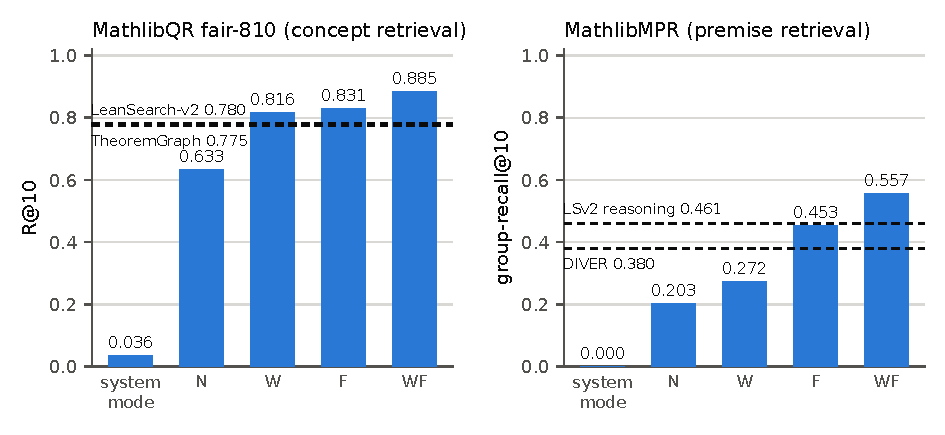
\includegraphics[width=\textwidth]{figures/fig3_retrieval}
\caption{Retrieval point estimates by system, with published anchors as
dashed reference lines. Left: MathlibQR fair-810 R@10 (anchors:
TheoremGraph 0.775, LeanSearch-v2 retriever+reranker 0.780). Right:
MathlibMPR group-recall@10 (anchors: LeanSearch-v2 reasoning 0.461, DIVER
0.380). System-mode is a single \code{brain\_bridge} call with no LLM;
N/W/F/WF are Sonnet agent arms; WF is the \textbf{post-hoc,
benchmark-informed} condition (\S6). The point estimates are unchanged from
version 1 (data: \code{bench/v2/score\_retrieval.py}); the confidence
intervals and significance tests were \emph{redone at the declaration level
for this edition} (\S6.1 declaration-cluster bootstrap, \S6.2 task
bootstrap) and are reported in the tables above, not drawn in this figure.}
\label{fig:retrieval}
\end{figure}

\subsection{Tool use under the manual}\label{sec:tooluse}

The census (pooled QR+MPR): F averages 2.2 calls/run; W 3.5
(decl\_exists 1{,}251 + brain\_bridge 608 --- verify-then-cite made
mechanical); WF 4.6 in a genuine dual-toolkit mix (decl\_grep
${\sim}$1.5k, decl\_exists ${\sim}$0.9k, brain\_bridge ${\sim}$0.7k,
decl\_read ${\sim}$0.5k, loogle ${\sim}$0.4k). Under the manual,
brain\_cell misuse (63\% failure rate in the v2 W-arm runs) falls to a
single call in WF. These are development observations about the same eval
set the manual was tuned on, and are labeled accordingly.

\begin{figure}[htbp]
\centering
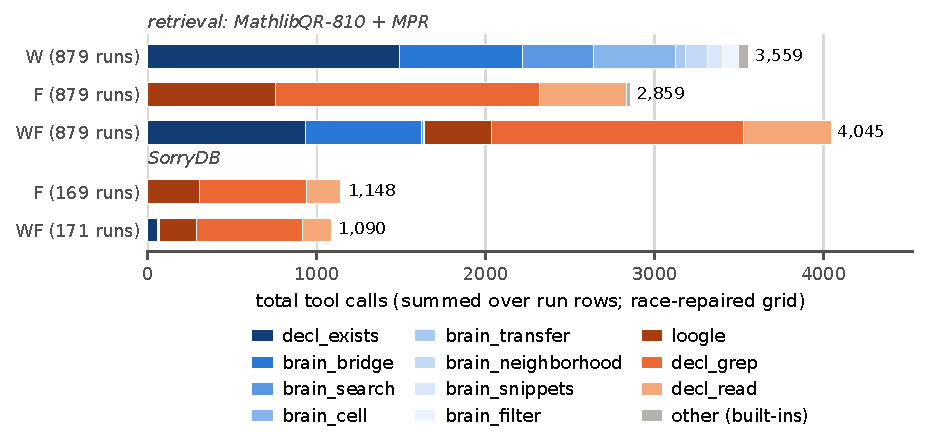
\includegraphics[width=\textwidth]{figures/fig5_tooluse}
\caption{Tool composition by arm: total calls summed over run rows
(retrieval pools QR-810 and MPR, 879 runs/arm; SorryDB ${\sim}$170
runs/arm). Blues are Brain tools, oranges formal-search tools, gray the
CLI's built-ins. \code{decl\_exists} dominates every Brain-bearing arm;
under the manual (WF --- the \textbf{post-hoc, benchmark-informed}
condition, \S6) the Brain toolkit contracts to
\code{brain\_bridge}\,+\,\code{decl\_exists} (\code{brain\_cell}: 482 calls
in W, one in WF); and on SorryDB the WF agent routes 94\% of its calls to
formal search (\S7). This telemetry is unchanged by this edition's
corrections. Data: \code{transcript\_stats.tool\_calls\_by\_name} summed
over \code{bench/v2/runs/}.}
\label{fig:tooluse}
\end{figure}

\begin{pendingbox}{Pending: bare-union (U) ablation (queued)}
\itshape
[[SLOT:UNION]] --- the bare-union U arm (W $\cup$ F tools, no manual;
\code{MANUAL\_ARMS} blanked in \code{bench/v2/run\_agent.py}) separates the
union effect from the briefing effect. Planned table on completion:
N / F / W / U / WF on both benchmarks, declaration-clustered (QR) and
task-bootstrap (MPR) CIs, with U-vs-F and WF-vs-U paired contrasts. Until
it lands, ``union tools'' and ``benchmark-informed manual'' remain
unseparated in WF.
\end{pendingbox}

\section{SorryDB: kernel-graded proving in live repositories
(claude-sonnet-5) [EXPLORATORY]}\label{sec:sorrydb}

SorryDB (arXiv:2603.02668, \url{https://sorrydb.org}) serves unsolved
\code{sorry}s from real Lean repositories; success is the repo
\emph{building} with your proof --- no judge anywhere, nothing to memorize.
Snapshot: the SorryDB-2601 1{,}000-task evaluation split.

\paragraph{Subset construction and the snapshot-rot finding.} Disk
permitted one repository build at a time, so we sampled repositories
rather than tasks. The original freeze --- 8 repositories, 164 tasks ---
lost \textbf{74 of 164 tasks (45\%)} in the ${\sim}$six months since the
snapshot: pinned commits of GlimpseOfLean, LeanCourse25, and most
Foundation and SemicircleLaw tasks no longer exist on GitHub (history
rewritten; unreachable commits deleted). No retrieval route worked, and
detection is subtle: GitHub's archive endpoint answers preflight HEAD for
dead commits with HTTP 200, so a liveness check that does not actually
fetch reports the pins healthy. Methodological finding: benchmarks pinned
to live repositories rot at the commit level, and the rot is invisible
unless every pin is re-fetched before use. The refreeze
(\code{bench/v2/sorrydb\_prep.py}, commit \code{db679e8d}) keeps only
verified-fetchable pins: \textbf{171 tasks across 10 repositories}.

\paragraph{Protocol.} Build-free, one-shot: each row carries the goal
state plus a $\pm$60-line window at the pinned commit; the agent (600\,s,
arms N/F/WF as in \S6) outputs one replacement for the \code{sorry}, with
an explicit honest-abstention rule. Verification
(\code{bench/v2/verify\_sorrydb.py}) clones at the pin, splices, rebuilds
the module; success = exit 0 with no sorry/axiom warning.

\paragraph{Results --- verdict-complete.} All 203 frozen-task candidate
proofs now have kernel verdicts (commit \code{9682b3b1}; the 8 curve25519
stragglers of v1 verified as 0 proved). Recomputed from
\code{bench/v2/runs/sorrydb/verify.jsonl} $\times$ the run rows, $n=171$
tasks/arm:

\begin{center}
\small
\begin{tabular}{@{}lccc@{}}
\toprule
 & N no tools & F formal & WF union+manual (post-hoc) \\
\midrule
run rows present & 168 & 169 & 171 \\
no output (timeout / no lean block) & 70 & 15 & 11 \\
honest give-up (literal \code{sorry}) & 40 & 83 & 86 \\
candidate proofs submitted & 58 & 71 & 74 \\
\best{proved (kernel)} & \best{2} & \best{9} & \best{10} \\
failed & 50 & 55 & 57 \\
unspliceable & 5 & 7 & 7 \\
verify timeout & 1 & 0 & 0 \\
\midrule
\best{proved / 171} & 1.2\% & 5.3\% & 5.8\% \\
Wilson 95\% CI & [0.3, 4.2] & [2.8, 9.7] & [3.2, 10.4] \\
repo-clustered boot 95\% CI & [0.0, 2.7] & [0.0, 10.7] & [0.0, 12.2] \\
proved / candidates & 3.4\% & 12.7\% & 13.5\% \\
total cost (USD) & \$58.97 & \$102.76 & \$108.87 \\
cost per proved & \$29.48 & \$11.42 & \$10.89 \\
mean wall-clock / task & 120\,s & 198\,s & 183\,s \\
\bottomrule
\end{tabular}
\end{center}

(3 N and 2 F tasks have no run row --- runner losses. Distinct sorries
proved across arms: 13; N's are a strict subset of both F's and WF's;
WF$\cap$F 6, WF-only 4, F-only 3. Proofs concentrate in 3 of the 10 repos:
PersistentDecomp, LeanAPAP, MiscYD.)

\paragraph{WF vs.\ F is statistically indistinguishable.} The point
difference is one proof (10 vs.\ 9 of 171): task-level exact McNemar 4/3,
\textbf{$p = 1.0$}; repo-clustered bootstrap difference $+0.58$pp, 95\% CI
$[+0.0, +1.85$pp$]$, with \textbf{34\% of resamples showing no difference
or worse} (\code{retrieval\_clustered.md} \S4). SorryDB provides
essentially no evidence about the Brain: WF routed 94\% of its tool calls
to formal search here, and no W-only or bare-union arm was run. What the
experiment does show is the tools-vs-no-tools gap --- N burns its budget
(70 of 168 rows produce nothing, mostly 600\,s timeouts) while tool arms
triple-to-quintuple the prove rate and double the honest-abstention rate
--- though with only 10 repo clusters even that deserves caution. The
cost-per-proved row is retained as bookkeeping; with 2/9/10 successes it is
unstable, and v1's ``adding the join never made the task more expensive per
success'' is deleted (\S9). The published SorryDB agentic best
(${\approx}30\%$) is not comparable: different task subset
(research-frontier-weighted) and materially different protocol (published
agents iterate against the build; ours drafted one-shot).

\section{What survives and what does not}\label{sec:survives}

Each retired v1 claim, paired with its v2 replacement.

{\footnotesize
\begin{longtable}{@{}p{0.36\textwidth}p{0.56\textwidth}@{}}
\toprule
v1 claim (retired) & v2 replacement (supported) \\
\midrule
\endfirsthead
\toprule
v1 claim (retired) & v2 replacement (supported) \\
\midrule
\endhead
\bottomrule
\endfoot
\bottomrule
\endlastfoot
``The join carries the effect'' (fresh McNemar $p<0.0001$) & The
\textbf{bundled Wikibrain condition} outperforms the tested controls:
completed-69 D 40.6\% vs.\ E 23.2\% ($p=0.023$, RD $+17.4$pp
$[+4.1,+30.7]$); post-repair full-100 42.0\% vs.\ 30.0\% ($p=0.073$, RD
$+12.0$pp $[+0.2,+23.8]$); D vs.\ C $p=0.0095$. Join-specific attribution
awaits the $2\times2$ factorial. \\
``42\% success'' & ``42\% \textbf{grounded typecheck rate}'' --- no
semantic-equivalence leg was graded; \S5 is the exploratory substitute. \\
``Contamination-proof / newer than every index'' &
``\textbf{Post-Brain-index}'': held out from the Brain's indexes only;
51/100 golds were exposed in arms C/E's checkout at run time. The leak's
direction favored C/E, and D's edge over E is strongest on unexposed tasks
(36.7\% vs.\ 8.2\%, $p=0.0026$) --- but D-vs-C is a null on that stratum. \\
``Arm E worst at 16\%; unjoined tool volume actively harmful'' & E's 31
no-output rows were session-limit 429s. Repaired, E is mid-pack at 30.0\%,
indistinguishable from C. \\
``WF sets the best rows we know of'' & A \textbf{post-hoc,
benchmark-informed} union+manual condition obtained the highest rows we
observed (QR 0.885, MPR 0.557); clustered CIs exclude the single-arm
baselines, but the manual was tuned on the same eval queries. \\
``Adding the join never made the task more expensive per success'' &
Deleted. Cost figures are descriptive; tokens-to-solve was never computed;
SorryDB's 10-vs-9 is $p=1.0$. \\
brain\_cell 63\% failure ``in the Tier-1 traces'' & The figure is from the
\textbf{v2 W-arm eval runs} (482 calls, 63.3\% failed). \\
\end{longtable}
}

What survives cleanly, with its register: the \textbf{hallucination
collapse} (D 6.8\% vs.\ 17.7--21.2\% fresh, post-repair;
checked-and-cited-anyway 13\% vs.\ 30--35\%) and its promotion to an
independent existence-verifier finding [preregistered-modified +
exploratory traces]; the \textbf{memorization quantification} (arm A
59.8\% $\to$ 20.0\%) [preregistered-modified]; the \textbf{system-mode gap}
(0.036 single-shot vs.\ 0.816 agentic on QR) --- an API deficiency, not a
content deficiency [exploratory]; the \textbf{F-matches-SOTA baseline} on
MPR (0.453 vs.\ 0.461) and the \textbf{concept$\neq$premise boundary}
(W $-$18pp) [exploratory]; the \textbf{snapshot-rot finding} (45\% of
pinned tasks unreachable in ${\sim}$6 months, invisible to HEAD-based
liveness checks) [exploratory]; and the \textbf{tools-vs-no-tools proving
gap} on SorryDB [exploratory, 10 clusters].

\section{Corrections and response to external review 1}\label{sec:corrections}

The review (\code{docs/research/review/REVIEW-1.md}, received 2026-07-27)
raised eight concerns. We verified every factual claim against the repo
before acting (\code{verification-of-review-1.json}); the table gives
concern $\to$ verification outcome $\to$ action taken in this edition.

{\footnotesize
\begin{longtable}{@{}p{0.02\textwidth}p{0.30\textwidth}p{0.16\textwidth}p{0.42\textwidth}@{}}
\toprule
\# & Concern & Verification & Action in v2 \\
\midrule
\endfirsthead
\toprule
\# & Concern & Verification & Action in v2 \\
\midrule
\endhead
\bottomrule
\endfoot
\bottomrule
\endlastfoot
1 & Tier-1 ``success'' does not measure semantic correctness (equivalence
grader is a stub) & CONFIRMED (the ``misleading'' characterization graded
PARTIAL --- v1's body disclosed the gap; its abstract did not) & Metric
renamed \textbf{grounded typecheck rate} everywhere including the abstract;
blind uncalibrated-judge pass launched as the exploratory substitute
(\S5); human calibration on the roadmap \\
2 & D vs.\ E does not isolate the join (D alone holds decl\_exists, which
optimizes a component of the score; 715 calls on fresh) & CONFIRMED &
``The join carries the effect'' retired; claims rewritten to ``the bundled
condition''; decl\_exists promoted to an independent finding (\S4.6);
$2\times2$ factorial is roadmap item 1 \\
3 & Arm E failed its manipulation check (4 informal calls vs.\ B's 345) &
CONFIRMED & Disclosed in \S3; yoked single-interface control on the
roadmap \\
4 & The fresh set was not isolated from formal-search sources (mutable
checkout at \code{61a5e4f338}; live Loogle unsnapshotted) & CONFIRMED
(64/100 basenames in-tree; 51 own-module) & Set renamed
\textbf{post-Brain-index}; exposure measured per-task and outcomes
stratified (\S4.4); frozen-snapshot protocol on the roadmap \\
5 & WF is test-set tuned (manual written after and from the same eval's
N/F/W results) & CONFIRMED (commit times 22:27 $\to$ 00:30 $\to$ 01:15;
every bracketed manual figure reproduces from the eval aggregates) & WF
labeled \textbf{post-hoc, benchmark-informed} at every mention including
the abstract; the manual's same-eval-set provenance stated plainly (\S6);
the v1 misattribution of the 63\% brain\_cell figure to Tier-1 corrected;
bare-union arm slotted; dev-set manual freeze on the roadmap \\
6 & Statistical independence and execution (810 QR rows are 171
declarations; sequential arm blocks; advisory turn budget; single seed; no
CIs) & CONFIRMED & Declaration-clustered QR reanalysis (\S6.1);
Wilson/bootstrap CIs on every rate; RD + CI on paired effects; sequential
blocks, overrun counts (C 50/D 38/E 32, max 88), and single-seed status
disclosed in \S3; row-level tests survive only as uncorrected footnotes \\
7 & The preregistered primary experiment was not completed, and the
deviations list did not say so & CONFIRMED & The complete execution table
(\S3) --- every component, status, inferential consequence; the
three-register labeling throughout; the zero-confirmatory statement in the
abstract and \S3 \\
8 & SorryDB provides little evidence about the join (no W-only/bare-union
arm; 94\% formal routing; missing verdicts; unstable cost-per-proof) &
CONFIRMED & All 203 candidate verdicts completed (\code{9682b3b1});
WF-vs-F stated as indistinguishable ($p=1.0$; 34\% of repo-bootstrap
resamples $\leq$0); repo-clustered CIs; the cost-per-success claim deleted \\
\end{longtable}
}

Two of the review's factual claims did not survive verification, recorded
here with appreciation rather than triumph --- the review's error rate
across 31 checked claims was two. First, MathlibMPR does not cluster by
PR: the data file has 69 tasks and 69 distinct PRs, one task each, so the
MPR analysis needed no cluster correction (the refuted claim). Second, arm
E's 31 declaration-less fresh runs were not a behavioral response to
interface overload --- they were contiguous session-limit 429 errors at the
tail of E's sequential block. That correction cuts both ways: it removes
the review's ``interface overload'' reading, and it removes v1's ``unjoined
volume is harmful'' claim along with the error-inflated headline
$p=2.4\times10^{-5}$ (which appears in this edition only in this paragraph,
as the corrected artifact it is; the repaired contrasts are \S4.2's).

\section{Roadmap}\label{sec:roadmap}

Adopted from the review's priority list, in its order:

\begin{enumerate}
\item \textbf{$2\times2$ factorial} --- \{join, no join\} $\times$
  \{decl\_exists, none\} on a truly frozen post-cutoff set, same tool
  counts and schemas; the experiment that turns \S4.6's attribution
  question into a measurement.
\item \textbf{Yoked unjoined control} --- one integrated interface
  returning equally concise informal and formal panels without declaring
  correspondences, plus a preregistered manipulation criterion for actual
  dual-corpus use.
\item \textbf{Manual freeze on development data} --- split MathlibQR by its
  171 target declarations, freeze the manual on a dev split, evaluate on
  unseen targets; run bare-union, F+manual, W+manual, union+manual.
\item \textbf{Human judge calibration} --- the preregistered 50-item
  hand-graded set, judge--human agreement reported, before any
  faithfulness number leaves the exploratory register.
\item \textbf{In-loop compiler proving} --- the SorryDB follow-up with
  identical build access per arm; external validity the one-shot protocol
  lacks.
\item \textbf{Multi-seed, multi-model} --- $\geq$3 seeds per task and a
  second model family; no variance estimate exists anywhere in the current
  data.
\item \textbf{Frozen search snapshots} --- read-only pinned checkout
  predating every test theorem, locally snapshotted Loogle index, per-run
  hashes of tree, index, Brain snapshot, prompts, and manifests.
\end{enumerate}

\section{Data availability}\label{sec:data}

{\sloppy
Everything needed to recompute this report lives in the private
preservation repository \textbf{\code{Deicyde/wikilean-bridge-experiment}}
(report at the root as \code{README.md} and under \code{report/}).
Provenance commits refer to the WikiLean working repository.\par}

{\footnotesize
\begin{longtable}{@{}p{0.34\textwidth}p{0.38\textwidth}p{0.20\textwidth}@{}}
\toprule
Path (preservation repo) & Contents & Key provenance commits (WikiLean) \\
\midrule
\endfirsthead
\toprule
Path (preservation repo) & Contents & Key provenance commits (WikiLean) \\
\midrule
\endhead
\bottomrule
\endfoot
\bottomrule
\endlastfoot
\code{docs/research/BRIDGE-EXPERIMENT.md} & preregistration incl.\ deviations 1--7 & \code{0d36f266} (2026-07-16) \\
\code{docs/research/BRIDGE-RESULTS.md} & Tier-1 + retrieval results log & \code{53f5cb31}, \code{daac6107} \\
\code{docs/research/review/} & external review 1 verbatim + independent claim-by-claim verification (29 confirmed / 1 partial / 1 refuted) & \code{f97e67e4} \\
\code{bench/*.py}, \code{bench/README.md}, \code{bench/arms/} & Tier-1 harness: runner, scorer, REPL typecheck rig, trace analysis, arm manifests & \code{068abe34}, \code{e554902e}, \code{6c2ca704}, \code{31b95caa}, \code{79ac3dfe} \\
\code{bench/data/bridge\_tasks.jsonl} (+\code{.stats}) & 371 ProofNet\# tasks; source pin + MIT licence & \code{e554902e}, \code{ec2a9e11} \\
\code{bench/data/fresh\_tasks.jsonl} (+\code{.stats}) & 100 post-Brain-index tasks + determinacy annotations + the (Brain-scoped) held-out check & \code{df5dbf92}, \code{a0d45103} \\
\code{bench/data/bridge\_summary.json} & v1 Tier-1 scored summary (pre-repair) & \code{53f5cb31} \\
\code{bench/data/runs/} & all 2{,}355 Tier-1 run rows, incl.\ the 31 repaired E rows & \code{19a90209} (repair driver) \\
\code{bench/data/runs\_E\_fresh\_429\_archive/} & the 31 original 429-errored E rows, byte-preserved & \code{f97e67e4} \\
\code{bench/data/runs\_devleak\_2026-07-18/} & the 120 quarantined skill-leak dev runs (deviation 6) & \code{f89e7a41} \\
\code{bench/analysis/} & v2 corrective statistics: \code{tier1\_reanalysis.\{py,json,md\}}, \code{fresh\_exposure.\{py,json,md\}}, \code{retrieval\_clustered.\{py,json,md\}}, \code{rerun\_E\_fresh.py}, \code{score\_e31\_v2.py} $\to$ \code{bridge\_summary\_v2.json} + \code{part1\_fresh100\_v2.\{json,md\}}, \code{judge\_fresh\_run.py} / \code{judge\_fresh\_summary.py} & \code{64c48052}, \code{19a90209} \\
\code{bench/v2/} & v2 harness + \code{AGENT\_MANUAL.md} & \code{c7629584}, \code{21032c06} \\
\code{bench/v2/data/} & MathlibQR/MPR (LeanSearch-v2 @\code{94f4888cbaf9}, CC BY 4.0), SorryDB-2601 split, \code{tasks\_frozen.jsonl} & \code{c7629584}, \code{87638cfc}, \code{db679e8d} \\
\code{bench/v2/runs/} & every v2 run row with full gzipped stream-json transcripts (QR 810$\times$4, MPR 69$\times$4, SorryDB 508 rows) + \code{verify.jsonl} --- \textbf{all 203 frozen-candidate kernel verdicts, complete} & \code{3664aa3d}, \code{daac6107}, \code{382e51bf}, \code{1fe21cca}, \code{9682b3b1} \\
\end{longtable}
}

{\sloppy
Recomputation entry points: \code{bench/score\_bridge.py} (Tier-1 grading),
\code{bench/analysis/tier1\_reanalysis.py} + \code{score\_e31\_v2.py}
(\S4), \code{bench/analysis/fresh\_exposure.py} (\S4.4),
\code{bench/analysis/retrieval\_clustered.py} (\S6.1--6.2, \S7
uncertainty), \code{bench/trace\_analysis.py} (\S4.5),
\code{bench/v2/score\_retrieval.py} (\S6 point estimates),
\code{bench/v2/verify\_sorrydb.py} (\S7 verdicts),
\code{bench/analysis/judge\_fresh\_summary.py} (\S5, pending).\par}

\paragraph{External sources cited} (fetched and verified during the v2
design sweep): TheoremGraph arXiv:2606.25363 $\cdot$ LeanSearch
arXiv:2403.13310 $\cdot$ LeanSearch-v2 arXiv:2605.13137 +
github.com/frenzymath/LeanSearch-v2 $\cdot$ LeanExplore arXiv:2506.11085
$\cdot$ SorryDB arXiv:2603.02668 + sorrydb.org $\cdot$ FATE
arXiv:2511.02872 $\cdot$ miniCTX arXiv:2408.03350 $\cdot$ LeanDojo
arXiv:2306.15626 $\cdot$ LeanAgent arXiv:2410.06209 $\cdot$
Numina-Lean-Agent arXiv:2601.14027 $\cdot$ miniF2F-v2 arXiv:2511.03108
$\cdot$ ProofNet\#/ProofNetVerif arXiv:2406.07222 $\cdot$ benchmark-faults
survey arXiv:2606.29493.

\appendix

\section{The agent manual}\label{app:manual}

\begin{quote}\itshape
The following is \code{bench/v2/AGENT\_MANUAL.md}, the briefing prepended
verbatim to every WF-arm prompt. It is reproduced unchanged as a study
artifact --- and, per \S6, it is a \textbf{post-hoc, benchmark-informed}
artifact: its bracketed figures were measured on the same MathlibQR/MPR
evaluation queries the WF arm was then scored on.
\end{quote}

\subsection*{Tool manual: searching Mathlib with the Brain + formal search}

You have two complementary toolkits. Every claim in this manual is measured
from ${\sim}5{,}500$ logged tool calls across 3{,}500 benchmark runs
(Tier-1 + Bridge v2); numbers in brackets are those measurements.

\subsection{The mental model}

\begin{itemize}
\item \textbf{The Brain (wikibrain, 8 tools)} is a \emph{curated knowledge
  graph} joining informal mathematics (Wikipedia/Wikidata concepts,
  external databases) to Mathlib declarations. It knows what things
  \emph{mean} and how concepts relate --- but it only ``atomizes''
  declarations that some concept, annotation, or tag claims (${\sim}$12k of
  Mathlib's declarations). It is a map, not the territory.
\item \textbf{Formal search (3 tools)} operates on \emph{all} of Mathlib
  directly: type-pattern search (loogle), source grep, source reading. It
  knows everything that exists but nothing about what it means informally.
\end{itemize}

Rule of thumb: \textbf{route by what you're holding.} Holding a concept
described in words $\to$ start with the Brain. Holding a type shape or name
fragment $\to$ start with formal search. Always finish with
\code{decl\_exists} on every name you intend to output.

\subsection{Formal search tools}

\subsubsection{\code{loogle}}
Type-pattern and constant search (the public \code{loogle.lean-lang.org}
service).
\begin{itemize}
\item USE for: ``a lemma whose statement looks like
  \code{\_ * \_ ${\leq}$ \_ * \_}'', searches by involved constants
  (\code{Real.sqrt}, \code{tsum}), name substrings.
\item Strengths: covers ALL of Mathlib; ${\sim}$0\% call errors [578 calls,
  0 errors]; the best premise-finding tool --- the loogle+grep toolkit
  matched a specialist premise retriever [group-recall@10 0.453 vs 0.461
  SOTA].
\item Weaknesses: needs Lean syntax fluency; a wrong pattern silently
  returns unrelated hits; small result payloads mean you often need
  decl\_read next.
\end{itemize}

\subsubsection{\code{decl\_grep}}
Regex search over the Mathlib source checkout (ripgrep).
\begin{itemize}
\item USE for: name fragments (``cantor''), notation, docstring phrases,
  finding the file a declaration lives in.
\item Strengths: the workhorse [1{,}206 calls, 0\% errors]; catches things
  loogle's type index can't (comments, docstrings, naming conventions).
\item Weaknesses: lexical only --- if the concept's name doesn't appear in
  source, grep cannot find it (descriptive queries like ``special case of
  X'' score worst for grep-based agents [nDCG 0.384 vs the Brain's 0.523]).
\end{itemize}

\subsubsection{\code{decl\_read}}
Read declaration source (with surrounding context) from the checkout.
\begin{itemize}
\item USE for: verifying a candidate actually says what you think BEFORE
  citing it; getting exact signatures and hypotheses.
\item Strengths: ground truth for any decl in Mathlib [397 calls, 0\%
  errors].
\item Weaknesses: you need the file/name first --- it is a confirmation
  tool, not a discovery tool.
\end{itemize}

\subsection{Brain tools}

\subsubsection{\code{brain\_bridge} --- THE ENTRY POINT for
informal$\to$formal}
Free text in, existence-verified declarations + owning atoms out, with
signatures, import lines, and one-hop dependency context.
\begin{itemize}
\item USE for: ``the concept described as $\langle$words$\rangle$'' ---
  especially nicknames and special-case descriptions, where the Brain's
  curated bonds beat grep [special\_case nDCG 0.523 vs 0.384; nickname
  0.779 vs 0.757].
\item CRITICAL LIMITATION (measured): its free-text matching is
  label/alias anchored, NOT semantic. A single call with a descriptive
  paraphrase usually misses [single-shot benchmark: 3.6\% R@10 vs 82\% for
  an agent that reformulates]. \textbf{Never accept one miss as the answer:
  reformulate 2--4 times} --- try the concept's canonical name, a synonym,
  the head noun alone. 8.9\% of calls return \code{match:"none"} [727
  calls]; that response includes nearest-candidate suggestions --- read
  them.
\item The \code{hits} list is existence-verified; bond quality matters:
  \code{exact} means the decl IS the concept; \code{formalizes}/weaker
  bonds are nearby.
\end{itemize}

\subsubsection{\code{brain\_search}}
Fuzzy label + alias search returning atoms (cells).
\begin{itemize}
\item USE for: resolving a name you half-know into an atom id; browsing
  what the Brain calls something [400 calls, 0\% errors --- the reliable
  fallback when brain\_bridge misses].
\item Weaknesses: returns atoms, not ranked decls --- follow with
  brain\_cell on the winning atom.
\end{itemize}

\subsubsection{\code{brain\_cell}}
The full atom card: Lean code, Wikidata description, DB snippets, organs.
\begin{itemize}
\item USE for: everything known about ONE object after bridge/search
  resolved it.
\item \textbf{THE \#1 MISUSE [63\% of 482 calls failed]: calling it with a
  bare \code{decl:Mathlib:Name} for an arbitrary declaration.} The Brain
  only has atoms for concept-joined decls; ``unresolvable key'' means
  \emph{no atom owns this decl}, NOT that the decl doesn't exist. For
  arbitrary decls use decl\_exists (works for all of Mathlib) and
  decl\_read for source. Call brain\_cell only with ids that came OUT of a
  Brain tool.
\end{itemize}

\subsubsection{\code{decl\_exists} --- THE DISCIPLINE TOOL}
Batch existence check for declaration names (backed by the full oracle ---
covers ALL of Mathlib, unlike brain\_cell).
\begin{itemize}
\item \textbf{USE ALWAYS, on every name you are about to output.} This is
  the measured difference between grounded and hallucinated citations:
  agents that verified before citing cut hallucinated-but-cited-anyway to
  13\% vs 33\% for agents relying on fuzzy search results alone. It is
  cheap [1{,}473 calls, 0.1\% errors] and batched --- check 10 names in one
  call.
\item Also returns verified-rename suggestions for stale names.
\end{itemize}

\subsubsection{\code{brain\_neighborhood}}
The synapse graph around an atom (depends/links/relates, cursored).
\begin{itemize}
\item USE for: ``what connects to X'' --- finding the connecting lemma
  between two concepts, walking dependencies.
\item Weaknesses: needs a valid atom id [24.8\% of calls errored --- same
  unresolvable-key trap as brain\_cell; resolve the atom first].
\end{itemize}

\subsubsection{\code{brain\_transfer} / \code{brain\_snippets} /
\code{brain\_filter}}
Narrower tools: label$\leftrightarrow$decl jumps for KNOWN labels
(transfer), stored source snippets (snippets), facet enumeration (filter).
High misuse rates when fed non-atom ids [40\%/57\% errors]. Prefer
brain\_bridge/brain\_search entry; reach for these only on ids the Brain
already returned.

\subsection{Routing playbook}

\begin{center}
\small
\begin{tabular}{@{}p{0.30\textwidth}p{0.62\textwidth}@{}}
\toprule
You are holding & Do this \\
\midrule
A concept in words & brain\_bridge $\to$ (miss?) reformulate $\to$
  brain\_search $\to$ brain\_cell \\
A special case / nickname & brain\_bridge (the Brain's best terrain) \\
A type shape & loogle \\
A name fragment & decl\_grep \\
Premises for a proof & loogle + decl\_grep FIRST [0.453 vs 0.272], Brain
  for concept grounding \\
A candidate name to cite & decl\_exists (batch, always) $\to$ decl\_read
  if the statement matters \\
An atom id from any Brain tool & brain\_cell / brain\_neighborhood freely \\
A bare decl name needing info & decl\_exists + decl\_read --- NOT
  brain\_cell \\
\bottomrule
\end{tabular}
\end{center}

\subsection{Anti-patterns (each one measured in prior runs)}

\begin{enumerate}
\item \textbf{Citing unverified names.} 33\% of hallucinated citations came
  from agents that had search evidence in front of them and cited a wrong
  name anyway. decl\_exists is binary and kills this.
\item \textbf{One query, then giving up.} The single-call miss rate on
  descriptive queries is ${\sim}$96\%; agents that reformulate reach
  ${\sim}$82\%. Iteration IS the algorithm.
\item \textbf{brain\_cell as a generic decl inspector.} 63\% failure rate.
  Brain atoms $\neq$ all of Mathlib.
\item \textbf{Answering outside the requested format.} 143/810 no-tool runs
  were scored 0 for exactly this. Re-read the output contract before
  replying.
\item \textbf{Inventing tool names} (e.g.\ \code{logue}, \code{lookie}).
  Use the names above.
\end{enumerate}

\end{document}
